
% Default to the notebook output style

    


% Inherit from the specified cell style.




    
\documentclass[11pt]{article}

    
    \usepackage{array}
    \usepackage[T1]{fontenc}
    % Nicer default font (+ math font) than Computer Modern for most use cases
    \usepackage{mathpazo}

    % Basic figure setup, for now with no caption control since it's done
    % automatically by Pandoc (which extracts ![](path) syntax from Markdown).
    \usepackage{graphicx}
    % We will generate all images so they have a width \maxwidth. This means
    % that they will get their normal width if they fit onto the page, but
    % are scaled down if they would overflow the margins.
    \makeatletter
    \def\maxwidth{\ifdim\Gin@nat@width>\linewidth\linewidth
    \else\Gin@nat@width\fi}
    \makeatother
    \let\Oldincludegraphics\includegraphics
    % Set max figure width to be 80% of text width, for now hardcoded.
    %\renewcommand{\includegraphics}[1]{\Oldincludegraphics[width=.8\maxwidth]{#1}}
    % Ensure that by default, figures have no caption (until we provide a
    % proper Figure object with a Caption API and a way to capture that
    % in the conversion process - todo).
    \usepackage{caption}
    \DeclareCaptionLabelFormat{nolabel}{}
    \captionsetup{labelformat=nolabel}

    \usepackage{adjustbox} % Used to constrain images to a maximum size 
    \usepackage{xcolor} % Allow colors to be defined
    \usepackage{enumerate} % Needed for markdown enumerations to work
    \usepackage{geometry} % Used to adjust the document margins
    \usepackage{amsmath} % Equations
    \usepackage{amssymb} % Equations
    \usepackage{textcomp} % defines textquotesingle
    % Hack from http://tex.stackexchange.com/a/47451/13684:
    \AtBeginDocument{%
        \def\PYZsq{\textquotesingle}% Upright quotes in Pygmentized code
    }
    \usepackage{upquote} % Upright quotes for verbatim code
    \usepackage{eurosym} % defines \euro
    \usepackage[mathletters]{ucs} % Extended unicode (utf-8) support
    \usepackage[utf8x]{inputenc} % Allow utf-8 characters in the tex document
    \usepackage{fancyvrb} % verbatim replacement that allows latex
    \usepackage{grffile} % extends the file name processing of package graphics 
                         % to support a larger range 
    % The hyperref package gives us a pdf with properly built
    % internal navigation ('pdf bookmarks' for the table of contents,
    % internal cross-reference links, web links for URLs, etc.)
    \usepackage{hyperref}
    \usepackage{longtable} % longtable support required by pandoc >1.10
    \usepackage{booktabs}  % table support for pandoc > 1.12.2
    \usepackage[inline]{enumitem} % IRkernel/repr support (it uses the enumerate* environment)
    \usepackage[normalem]{ulem} % ulem is needed to support strikethroughs (\sout)
                                % normalem makes italics be italics, not underlines
    \usepackage{mathrsfs}
    

    
    
    % Colors for the hyperref package
    \definecolor{urlcolor}{rgb}{0,.145,.698}
    \definecolor{linkcolor}{rgb}{.71,0.21,0.01}
    \definecolor{citecolor}{rgb}{.12,.54,.11}

    % ANSI colors
    \definecolor{ansi-black}{HTML}{3E424D}
    \definecolor{ansi-black-intense}{HTML}{282C36}
    \definecolor{ansi-red}{HTML}{E75C58}
    \definecolor{ansi-red-intense}{HTML}{B22B31}
    \definecolor{ansi-green}{HTML}{00A250}
    \definecolor{ansi-green-intense}{HTML}{007427}
    \definecolor{ansi-yellow}{HTML}{DDB62B}
    \definecolor{ansi-yellow-intense}{HTML}{B27D12}
    \definecolor{ansi-blue}{HTML}{208FFB}
    \definecolor{ansi-blue-intense}{HTML}{0065CA}
    \definecolor{ansi-magenta}{HTML}{D160C4}
    \definecolor{ansi-magenta-intense}{HTML}{A03196}
    \definecolor{ansi-cyan}{HTML}{60C6C8}
    \definecolor{ansi-cyan-intense}{HTML}{258F8F}
    \definecolor{ansi-white}{HTML}{C5C1B4}
    \definecolor{ansi-white-intense}{HTML}{A1A6B2}
    \definecolor{ansi-default-inverse-fg}{HTML}{FFFFFF}
    \definecolor{ansi-default-inverse-bg}{HTML}{000000}

    % commands and environments needed by pandoc snippets
    % extracted from the output of `pandoc -s`
    \providecommand{\tightlist}{%
      \setlength{\itemsep}{0pt}\setlength{\parskip}{0pt}}
    \DefineVerbatimEnvironment{Highlighting}{Verbatim}{commandchars=\\\{\}}
    % Add ',fontsize=\small' for more characters per line
    \newenvironment{Shaded}{}{}
    \newcommand{\KeywordTok}[1]{\textcolor[rgb]{0.00,0.44,0.13}{\textbf{{#1}}}}
    \newcommand{\DataTypeTok}[1]{\textcolor[rgb]{0.56,0.13,0.00}{{#1}}}
    \newcommand{\DecValTok}[1]{\textcolor[rgb]{0.25,0.63,0.44}{{#1}}}
    \newcommand{\BaseNTok}[1]{\textcolor[rgb]{0.25,0.63,0.44}{{#1}}}
    \newcommand{\FloatTok}[1]{\textcolor[rgb]{0.25,0.63,0.44}{{#1}}}
    \newcommand{\CharTok}[1]{\textcolor[rgb]{0.25,0.44,0.63}{{#1}}}
    \newcommand{\StringTok}[1]{\textcolor[rgb]{0.25,0.44,0.63}{{#1}}}
    \newcommand{\CommentTok}[1]{\textcolor[rgb]{0.38,0.63,0.69}{\textit{{#1}}}}
    \newcommand{\OtherTok}[1]{\textcolor[rgb]{0.00,0.44,0.13}{{#1}}}
    \newcommand{\AlertTok}[1]{\textcolor[rgb]{1.00,0.00,0.00}{\textbf{{#1}}}}
    \newcommand{\FunctionTok}[1]{\textcolor[rgb]{0.02,0.16,0.49}{{#1}}}
    \newcommand{\RegionMarkerTok}[1]{{#1}}
    \newcommand{\ErrorTok}[1]{\textcolor[rgb]{1.00,0.00,0.00}{\textbf{{#1}}}}
    \newcommand{\NormalTok}[1]{{#1}}
    
    % Additional commands for more recent versions of Pandoc
    \newcommand{\ConstantTok}[1]{\textcolor[rgb]{0.53,0.00,0.00}{{#1}}}
    \newcommand{\SpecialCharTok}[1]{\textcolor[rgb]{0.25,0.44,0.63}{{#1}}}
    \newcommand{\VerbatimStringTok}[1]{\textcolor[rgb]{0.25,0.44,0.63}{{#1}}}
    \newcommand{\SpecialStringTok}[1]{\textcolor[rgb]{0.73,0.40,0.53}{{#1}}}
    \newcommand{\ImportTok}[1]{{#1}}
    \newcommand{\DocumentationTok}[1]{\textcolor[rgb]{0.73,0.13,0.13}{\textit{{#1}}}}
    \newcommand{\AnnotationTok}[1]{\textcolor[rgb]{0.38,0.63,0.69}{\textbf{\textit{{#1}}}}}
    \newcommand{\CommentVarTok}[1]{\textcolor[rgb]{0.38,0.63,0.69}{\textbf{\textit{{#1}}}}}
    \newcommand{\VariableTok}[1]{\textcolor[rgb]{0.10,0.09,0.49}{{#1}}}
    \newcommand{\ControlFlowTok}[1]{\textcolor[rgb]{0.00,0.44,0.13}{\textbf{{#1}}}}
    \newcommand{\OperatorTok}[1]{\textcolor[rgb]{0.40,0.40,0.40}{{#1}}}
    \newcommand{\BuiltInTok}[1]{{#1}}
    \newcommand{\ExtensionTok}[1]{{#1}}
    \newcommand{\PreprocessorTok}[1]{\textcolor[rgb]{0.74,0.48,0.00}{{#1}}}
    \newcommand{\AttributeTok}[1]{\textcolor[rgb]{0.49,0.56,0.16}{{#1}}}
    \newcommand{\InformationTok}[1]{\textcolor[rgb]{0.38,0.63,0.69}{\textbf{\textit{{#1}}}}}
    \newcommand{\WarningTok}[1]{\textcolor[rgb]{0.38,0.63,0.69}{\textbf{\textit{{#1}}}}}
    
    
    % Define a nice break command that doesn't care if a line doesn't already
    % exist.
    \def\br{\hspace*{\fill} \\* }
    % Math Jax compatibility definitions
    \def\gt{>}
    \def\lt{<}
    \let\Oldtex\TeX
    \let\Oldlatex\LaTeX
    \renewcommand{\TeX}{\textrm{\Oldtex}}
    \renewcommand{\LaTeX}{\textrm{\Oldlatex}}
    % Document parameters
    % Document title
    \title{Credit Default Swaps - Practical Lesson 7}
    \author {Matteo Sani\\ \href{mailto:matteosan1@gmail.com}{matteosan1@gmail.com}}
    
    
    
    
    

    % Pygments definitions
    
\makeatletter
\def\PY@reset{\let\PY@it=\relax \let\PY@bf=\relax%
    \let\PY@ul=\relax \let\PY@tc=\relax%
    \let\PY@bc=\relax \let\PY@ff=\relax}
\def\PY@tok#1{\csname PY@tok@#1\endcsname}
\def\PY@toks#1+{\ifx\relax#1\empty\else%
    \PY@tok{#1}\expandafter\PY@toks\fi}
\def\PY@do#1{\PY@bc{\PY@tc{\PY@ul{%
    \PY@it{\PY@bf{\PY@ff{#1}}}}}}}
\def\PY#1#2{\PY@reset\PY@toks#1+\relax+\PY@do{#2}}

\expandafter\def\csname PY@tok@w\endcsname{\def\PY@tc##1{\textcolor[rgb]{0.73,0.73,0.73}{##1}}}
\expandafter\def\csname PY@tok@c\endcsname{\let\PY@it=\textit\def\PY@tc##1{\textcolor[rgb]{0.25,0.50,0.50}{##1}}}
\expandafter\def\csname PY@tok@cp\endcsname{\def\PY@tc##1{\textcolor[rgb]{0.74,0.48,0.00}{##1}}}
\expandafter\def\csname PY@tok@k\endcsname{\let\PY@bf=\textbf\def\PY@tc##1{\textcolor[rgb]{0.00,0.50,0.00}{##1}}}
\expandafter\def\csname PY@tok@kp\endcsname{\def\PY@tc##1{\textcolor[rgb]{0.00,0.50,0.00}{##1}}}
\expandafter\def\csname PY@tok@kt\endcsname{\def\PY@tc##1{\textcolor[rgb]{0.69,0.00,0.25}{##1}}}
\expandafter\def\csname PY@tok@o\endcsname{\def\PY@tc##1{\textcolor[rgb]{0.40,0.40,0.40}{##1}}}
\expandafter\def\csname PY@tok@ow\endcsname{\let\PY@bf=\textbf\def\PY@tc##1{\textcolor[rgb]{0.67,0.13,1.00}{##1}}}
\expandafter\def\csname PY@tok@nb\endcsname{\def\PY@tc##1{\textcolor[rgb]{0.00,0.50,0.00}{##1}}}
\expandafter\def\csname PY@tok@nf\endcsname{\def\PY@tc##1{\textcolor[rgb]{0.00,0.00,1.00}{##1}}}
\expandafter\def\csname PY@tok@nc\endcsname{\let\PY@bf=\textbf\def\PY@tc##1{\textcolor[rgb]{0.00,0.00,1.00}{##1}}}
\expandafter\def\csname PY@tok@nn\endcsname{\let\PY@bf=\textbf\def\PY@tc##1{\textcolor[rgb]{0.00,0.00,1.00}{##1}}}
\expandafter\def\csname PY@tok@ne\endcsname{\let\PY@bf=\textbf\def\PY@tc##1{\textcolor[rgb]{0.82,0.25,0.23}{##1}}}
\expandafter\def\csname PY@tok@nv\endcsname{\def\PY@tc##1{\textcolor[rgb]{0.10,0.09,0.49}{##1}}}
\expandafter\def\csname PY@tok@no\endcsname{\def\PY@tc##1{\textcolor[rgb]{0.53,0.00,0.00}{##1}}}
\expandafter\def\csname PY@tok@nl\endcsname{\def\PY@tc##1{\textcolor[rgb]{0.63,0.63,0.00}{##1}}}
\expandafter\def\csname PY@tok@ni\endcsname{\let\PY@bf=\textbf\def\PY@tc##1{\textcolor[rgb]{0.60,0.60,0.60}{##1}}}
\expandafter\def\csname PY@tok@na\endcsname{\def\PY@tc##1{\textcolor[rgb]{0.49,0.56,0.16}{##1}}}
\expandafter\def\csname PY@tok@nt\endcsname{\let\PY@bf=\textbf\def\PY@tc##1{\textcolor[rgb]{0.00,0.50,0.00}{##1}}}
\expandafter\def\csname PY@tok@nd\endcsname{\def\PY@tc##1{\textcolor[rgb]{0.67,0.13,1.00}{##1}}}
\expandafter\def\csname PY@tok@s\endcsname{\def\PY@tc##1{\textcolor[rgb]{0.73,0.13,0.13}{##1}}}
\expandafter\def\csname PY@tok@sd\endcsname{\let\PY@it=\textit\def\PY@tc##1{\textcolor[rgb]{0.73,0.13,0.13}{##1}}}
\expandafter\def\csname PY@tok@si\endcsname{\let\PY@bf=\textbf\def\PY@tc##1{\textcolor[rgb]{0.73,0.40,0.53}{##1}}}
\expandafter\def\csname PY@tok@se\endcsname{\let\PY@bf=\textbf\def\PY@tc##1{\textcolor[rgb]{0.73,0.40,0.13}{##1}}}
\expandafter\def\csname PY@tok@sr\endcsname{\def\PY@tc##1{\textcolor[rgb]{0.73,0.40,0.53}{##1}}}
\expandafter\def\csname PY@tok@ss\endcsname{\def\PY@tc##1{\textcolor[rgb]{0.10,0.09,0.49}{##1}}}
\expandafter\def\csname PY@tok@sx\endcsname{\def\PY@tc##1{\textcolor[rgb]{0.00,0.50,0.00}{##1}}}
\expandafter\def\csname PY@tok@m\endcsname{\def\PY@tc##1{\textcolor[rgb]{0.40,0.40,0.40}{##1}}}
\expandafter\def\csname PY@tok@gh\endcsname{\let\PY@bf=\textbf\def\PY@tc##1{\textcolor[rgb]{0.00,0.00,0.50}{##1}}}
\expandafter\def\csname PY@tok@gu\endcsname{\let\PY@bf=\textbf\def\PY@tc##1{\textcolor[rgb]{0.50,0.00,0.50}{##1}}}
\expandafter\def\csname PY@tok@gd\endcsname{\def\PY@tc##1{\textcolor[rgb]{0.63,0.00,0.00}{##1}}}
\expandafter\def\csname PY@tok@gi\endcsname{\def\PY@tc##1{\textcolor[rgb]{0.00,0.63,0.00}{##1}}}
\expandafter\def\csname PY@tok@gr\endcsname{\def\PY@tc##1{\textcolor[rgb]{1.00,0.00,0.00}{##1}}}
\expandafter\def\csname PY@tok@ge\endcsname{\let\PY@it=\textit}
\expandafter\def\csname PY@tok@gs\endcsname{\let\PY@bf=\textbf}
\expandafter\def\csname PY@tok@gp\endcsname{\let\PY@bf=\textbf\def\PY@tc##1{\textcolor[rgb]{0.00,0.00,0.50}{##1}}}
\expandafter\def\csname PY@tok@go\endcsname{\def\PY@tc##1{\textcolor[rgb]{0.53,0.53,0.53}{##1}}}
\expandafter\def\csname PY@tok@gt\endcsname{\def\PY@tc##1{\textcolor[rgb]{0.00,0.27,0.87}{##1}}}
\expandafter\def\csname PY@tok@err\endcsname{\def\PY@bc##1{\setlength{\fboxsep}{0pt}\fcolorbox[rgb]{1.00,0.00,0.00}{1,1,1}{\strut ##1}}}
\expandafter\def\csname PY@tok@kc\endcsname{\let\PY@bf=\textbf\def\PY@tc##1{\textcolor[rgb]{0.00,0.50,0.00}{##1}}}
\expandafter\def\csname PY@tok@kd\endcsname{\let\PY@bf=\textbf\def\PY@tc##1{\textcolor[rgb]{0.00,0.50,0.00}{##1}}}
\expandafter\def\csname PY@tok@kn\endcsname{\let\PY@bf=\textbf\def\PY@tc##1{\textcolor[rgb]{0.00,0.50,0.00}{##1}}}
\expandafter\def\csname PY@tok@kr\endcsname{\let\PY@bf=\textbf\def\PY@tc##1{\textcolor[rgb]{0.00,0.50,0.00}{##1}}}
\expandafter\def\csname PY@tok@bp\endcsname{\def\PY@tc##1{\textcolor[rgb]{0.00,0.50,0.00}{##1}}}
\expandafter\def\csname PY@tok@fm\endcsname{\def\PY@tc##1{\textcolor[rgb]{0.00,0.00,1.00}{##1}}}
\expandafter\def\csname PY@tok@vc\endcsname{\def\PY@tc##1{\textcolor[rgb]{0.10,0.09,0.49}{##1}}}
\expandafter\def\csname PY@tok@vg\endcsname{\def\PY@tc##1{\textcolor[rgb]{0.10,0.09,0.49}{##1}}}
\expandafter\def\csname PY@tok@vi\endcsname{\def\PY@tc##1{\textcolor[rgb]{0.10,0.09,0.49}{##1}}}
\expandafter\def\csname PY@tok@vm\endcsname{\def\PY@tc##1{\textcolor[rgb]{0.10,0.09,0.49}{##1}}}
\expandafter\def\csname PY@tok@sa\endcsname{\def\PY@tc##1{\textcolor[rgb]{0.73,0.13,0.13}{##1}}}
\expandafter\def\csname PY@tok@sb\endcsname{\def\PY@tc##1{\textcolor[rgb]{0.73,0.13,0.13}{##1}}}
\expandafter\def\csname PY@tok@sc\endcsname{\def\PY@tc##1{\textcolor[rgb]{0.73,0.13,0.13}{##1}}}
\expandafter\def\csname PY@tok@dl\endcsname{\def\PY@tc##1{\textcolor[rgb]{0.73,0.13,0.13}{##1}}}
\expandafter\def\csname PY@tok@s2\endcsname{\def\PY@tc##1{\textcolor[rgb]{0.73,0.13,0.13}{##1}}}
\expandafter\def\csname PY@tok@sh\endcsname{\def\PY@tc##1{\textcolor[rgb]{0.73,0.13,0.13}{##1}}}
\expandafter\def\csname PY@tok@s1\endcsname{\def\PY@tc##1{\textcolor[rgb]{0.73,0.13,0.13}{##1}}}
\expandafter\def\csname PY@tok@mb\endcsname{\def\PY@tc##1{\textcolor[rgb]{0.40,0.40,0.40}{##1}}}
\expandafter\def\csname PY@tok@mf\endcsname{\def\PY@tc##1{\textcolor[rgb]{0.40,0.40,0.40}{##1}}}
\expandafter\def\csname PY@tok@mh\endcsname{\def\PY@tc##1{\textcolor[rgb]{0.40,0.40,0.40}{##1}}}
\expandafter\def\csname PY@tok@mi\endcsname{\def\PY@tc##1{\textcolor[rgb]{0.40,0.40,0.40}{##1}}}
\expandafter\def\csname PY@tok@il\endcsname{\def\PY@tc##1{\textcolor[rgb]{0.40,0.40,0.40}{##1}}}
\expandafter\def\csname PY@tok@mo\endcsname{\def\PY@tc##1{\textcolor[rgb]{0.40,0.40,0.40}{##1}}}
\expandafter\def\csname PY@tok@ch\endcsname{\let\PY@it=\textit\def\PY@tc##1{\textcolor[rgb]{0.25,0.50,0.50}{##1}}}
\expandafter\def\csname PY@tok@cm\endcsname{\let\PY@it=\textit\def\PY@tc##1{\textcolor[rgb]{0.25,0.50,0.50}{##1}}}
\expandafter\def\csname PY@tok@cpf\endcsname{\let\PY@it=\textit\def\PY@tc##1{\textcolor[rgb]{0.25,0.50,0.50}{##1}}}
\expandafter\def\csname PY@tok@c1\endcsname{\let\PY@it=\textit\def\PY@tc##1{\textcolor[rgb]{0.25,0.50,0.50}{##1}}}
\expandafter\def\csname PY@tok@cs\endcsname{\let\PY@it=\textit\def\PY@tc##1{\textcolor[rgb]{0.25,0.50,0.50}{##1}}}

\def\PYZbs{\char`\\}
\def\PYZus{\char`\_}
\def\PYZob{\char`\{}
\def\PYZcb{\char`\}}
\def\PYZca{\char`\^}
\def\PYZam{\char`\&}
\def\PYZlt{\char`\<}
\def\PYZgt{\char`\>}
\def\PYZsh{\char`\#}
\def\PYZpc{\char`\%}
\def\PYZdl{\char`\$}
\def\PYZhy{\char`\-}
\def\PYZsq{\char`\'}
\def\PYZdq{\char`\"}
\def\PYZti{\char`\~}
% for compatibility with earlier versions
\def\PYZat{@}
\def\PYZlb{[}
\def\PYZrb{]}
\makeatother


    % Exact colors from NB
    \definecolor{incolor}{rgb}{0.0, 0.0, 0.5}
    \definecolor{outcolor}{rgb}{0.545, 0.0, 0.0}



    
    % Prevent overflowing lines due to hard-to-break entities
    \sloppy 
    % Setup hyperref package
    \hypersetup{
      breaklinks=true,  % so long urls are correctly broken across lines
      colorlinks=true,
      urlcolor=urlcolor,
      linkcolor=linkcolor,
      citecolor=citecolor,
      }
    % Slightly bigger margins than the latex defaults
    
    \geometry{verbose,tmargin=1in,bmargin=1in,lmargin=1in,rmargin=1in}
    
    

    \begin{document}
    
    
    \maketitle
    
    

    
    \hypertarget{credit-default-swaps---practical-lesson-7}{%
\section{Catching up}\label{credit-default-swaps---practical-lesson-7}}

\hypertarget{updating-the-finmarkets-module}{%
\subsection{\texorpdfstring{Updating the \texttt{finmarkets}
Module}{Updating the finmarkets Module}}\label{updating-the-finmarkets-module}}

Before going on talking about credit curves let's update our financial
module by adding the objects we derived in the latest lectures:

\begin{itemize}
\tightlist
\item
  update the \texttt{generate\_swap\_dates} function for generic tenors
\item
  \texttt{ForwardRateCurve} class
\item
  \texttt{InterestRateSwap} class
\item
  \texttt{InterestRateSwaption} class with two attributes (exercise date
  and irs instanciation) and two methods two compute npv with
  Black-Scholes formula or by MC simulation
\end{itemize}

    \begin{Verbatim}[commandchars=\\\{\}]
{\color{incolor}In [{\color{incolor}1}]:} \PY{k}{class} \PY{n+nc}{InterestRateSwaption}\PY{p}{:}
            
            \PY{k}{def} \PY{n+nf}{\PYZus{}\PYZus{}init\PYZus{}\PYZus{}}\PY{p}{(}\PY{n+nb+bp}{self}\PY{p}{,} \PY{n}{exercise\PYZus{}date}\PY{p}{,} \PY{n}{irs}\PY{p}{)}\PY{p}{:}
                \PY{n+nb+bp}{self}\PY{o}{.}\PY{n}{exercise\PYZus{}date} \PY{o}{=} \PY{n}{exercise\PYZus{}date}
                \PY{n+nb+bp}{self}\PY{o}{.}\PY{n}{irs} \PY{o}{=} \PY{n}{irs}
                
            \PY{k}{def} \PY{n+nf}{npv\PYZus{}bs}\PY{p}{(}\PY{n+nb+bp}{self}\PY{p}{,} \PY{n}{discount\PYZus{}curve}\PY{p}{,} \PY{n}{libor\PYZus{}curve}\PY{p}{,} \PY{n}{sigma}\PY{p}{)}\PY{p}{:}
                
                \PY{n}{A} \PY{o}{=} \PY{n+nb+bp}{self}\PY{o}{.}\PY{n}{irs}\PY{o}{.}\PY{n}{annuity}\PY{p}{(}\PY{n}{discount\PYZus{}curve}\PY{p}{)}
                \PY{n}{S} \PY{o}{=} \PY{n+nb+bp}{self}\PY{o}{.}\PY{n}{irs}\PY{o}{.}\PY{n}{swap\PYZus{}rate}\PY{p}{(}\PY{n}{discount\PYZus{}curve}\PY{p}{,} \PY{n}{libor\PYZus{}curve}\PY{p}{)}
        
                \PY{n}{T} \PY{o}{=} \PY{p}{(}\PY{n+nb+bp}{self}\PY{o}{.}\PY{n}{exercise\PYZus{}date} \PY{o}{\PYZhy{}} \PY{n}{discount\PYZus{}curve}\PY{o}{.}\PY{n}{today}\PY{p}{)}\PY{o}{.}\PY{n}{days} \PY{o}{/} \PY{l+m+mi}{365}
        
                \PY{n}{d1} \PY{o}{=} \PY{p}{(}\PY{n}{math}\PY{o}{.}\PY{n}{log}\PY{p}{(}\PY{n}{S}\PY{o}{/}\PY{n+nb+bp}{self}\PY{o}{.}\PY{n}{irs}\PY{o}{.}\PY{n}{fixed\PYZus{}rate}\PY{p}{)} \PY{o}{+} \PY{l+m+mf}{0.5} \PY{o}{*} \PY{n}{sigma}\PY{o}{*}\PY{o}{*}\PY{l+m+mi}{2} \PY{o}{*} \PY{n}{T}\PY{p}{)} \PY{o}{/} \PY{p}{(}\PY{n}{sigma} \PY{o}{*} \PY{n}{T}\PY{o}{*}\PY{o}{*}\PY{l+m+mf}{0.5}\PY{p}{)}
                \PY{n}{d2} \PY{o}{=} \PY{n}{d1} \PY{o}{\PYZhy{}} \PY{p}{(}\PY{n}{sigma} \PY{o}{*} \PY{n}{T}\PY{o}{*}\PY{o}{*}\PY{l+m+mf}{0.5}\PY{p}{)}
        
                \PY{n}{npv} \PY{o}{=} \PY{n+nb+bp}{self}\PY{o}{.}\PY{n}{irs}\PY{o}{.}\PY{n}{notional} \PY{o}{*} \PY{n}{A} \PY{o}{*} \PY{p}{(}\PY{n}{S} \PY{o}{*} \PY{n}{scipy}\PY{o}{.}\PY{n}{stats}\PY{o}{.}\PY{n}{norm}\PY{o}{.}\PY{n}{cdf}\PY{p}{(}\PY{n}{d1}\PY{p}{)} \PY{o}{\PYZhy{}} 
                                               \PY{n+nb+bp}{self}\PY{o}{.}\PY{n}{irs}\PY{o}{.}\PY{n}{fixed\PYZus{}rate} \PY{o}{*} \PY{n}{scipy}\PY{o}{.}\PY{n}{stats}\PY{o}{.}\PY{n}{norm}\PY{o}{.}\PY{n}{cdf}\PY{p}{(}\PY{n}{d2}\PY{p}{)}\PY{p}{)}
                
                \PY{k}{return} \PY{n}{npv}
            
            \PY{k}{def} \PY{n+nf}{npv\PYZus{}mc}\PY{p}{(}\PY{n+nb+bp}{self}\PY{p}{,} \PY{n}{discount\PYZus{}curve}\PY{p}{,} \PY{n}{libor\PYZus{}curve}\PY{p}{,} \PY{n}{sigma}\PY{p}{,} \PY{n}{n\PYZus{}scenarios}\PY{o}{=}\PY{l+m+mi}{10000}\PY{p}{)}\PY{p}{:}
                
                \PY{n}{A} \PY{o}{=} \PY{n+nb+bp}{self}\PY{o}{.}\PY{n}{irs}\PY{o}{.}\PY{n}{annuity}\PY{p}{(}\PY{n}{discount\PYZus{}curve}\PY{p}{)}
                \PY{n}{S} \PY{o}{=} \PY{n+nb+bp}{self}\PY{o}{.}\PY{n}{irs}\PY{o}{.}\PY{n}{swap\PYZus{}rate}\PY{p}{(}\PY{n}{discount\PYZus{}curve}\PY{p}{,} \PY{n}{libor\PYZus{}curve}\PY{p}{)}
        
                \PY{n}{T} \PY{o}{=} \PY{p}{(}\PY{n+nb+bp}{self}\PY{o}{.}\PY{n}{exercise\PYZus{}date} \PY{o}{\PYZhy{}} \PY{n}{discount\PYZus{}curve}\PY{o}{.}\PY{n}{today}\PY{p}{)}\PY{o}{.}\PY{n}{days} \PY{o}{/} \PY{l+m+mi}{365}
                \PY{n}{discounted\PYZus{}payoffs} \PY{o}{=} \PY{p}{[}\PY{p}{]}
        
                \PY{k}{for} \PY{n}{i\PYZus{}scenario} \PY{o+ow}{in} \PY{n+nb}{range}\PY{p}{(}\PY{n}{n\PYZus{}scenarios}\PY{p}{)}\PY{p}{:}
                    \PY{n}{S\PYZus{}simulated} \PY{o}{=} \PY{n}{S} \PY{o}{*} \PY{n}{math}\PY{o}{.}\PY{n}{exp}\PY{p}{(}\PY{o}{\PYZhy{}}\PY{l+m+mf}{0.5} \PY{o}{*} \PY{n}{sigma} \PY{o}{*} \PY{n}{sigma} \PY{o}{*} \PY{n}{T} \PY{o}{+}
                                               \PY{n}{sigma} \PY{o}{*} \PY{n}{math}\PY{o}{.}\PY{n}{sqrt}\PY{p}{(}\PY{n}{T}\PY{p}{)} \PY{o}{*} \PY{n}{numpy}\PY{o}{.}\PY{n}{random}\PY{o}{.}\PY{n}{normal}\PY{p}{(}\PY{p}{)}\PY{p}{)}
        
                    \PY{n}{swap\PYZus{}npv} \PY{o}{=} \PY{n+nb+bp}{self}\PY{o}{.}\PY{n}{irs}\PY{o}{.}\PY{n}{notional} \PY{o}{*} \PY{p}{(}\PY{n}{S\PYZus{}simulated} \PY{o}{\PYZhy{}} \PY{n+nb+bp}{self}\PY{o}{.}\PY{n}{irs}\PY{o}{.}\PY{n}{fixed\PYZus{}rate}\PY{p}{)} \PY{o}{*} \PY{n}{A}
                    \PY{n}{discounted\PYZus{}payoffs}\PY{o}{.}\PY{n}{append}\PY{p}{(}\PY{n+nb}{max}\PY{p}{(}\PY{l+m+mi}{0}\PY{p}{,} \PY{n}{swap\PYZus{}npv}\PY{p}{)}\PY{p}{)}
        
                \PY{n}{npv\PYZus{}mc} \PY{o}{=} \PY{n}{numpy}\PY{o}{.}\PY{n}{mean}\PY{p}{(}\PY{n}{discounted\PYZus{}payoffs}\PY{p}{)}
                \PY{n}{npv\PYZus{}error} \PY{o}{=} \PY{l+m+mi}{3} \PY{o}{*} \PY{n}{numpy}\PY{o}{.}\PY{n}{std}\PY{p}{(}\PY{n}{discounted\PYZus{}payoffs}\PY{p}{)} \PY{o}{/} \PY{n}{math}\PY{o}{.}\PY{n}{sqrt}\PY{p}{(}\PY{n}{n\PYZus{}scenarios}\PY{p}{)}
                
                \PY{k}{return} \PY{n}{npv\PYZus{}mc}\PY{p}{,} \PY{n}{npv\PYZus{}error}
\end{Verbatim}

    \begin{Verbatim}[commandchars=\\\{\}]
{\color{incolor}In [{\color{incolor}2}]:} \PY{k+kn}{import} \PY{n+nn}{finmarkets}
        \PY{n+nb}{dir}\PY{p}{(}\PY{n}{finmarkets}\PY{p}{)}
\end{Verbatim}

\begin{Verbatim}[commandchars=\\\{\}]
{\color{outcolor}Out[{\color{outcolor}2}]:} ['DiscountCurve',
         'ForwardRateCurve',
         'InterestRateSwap',
         'InterestRateSwaption',
         'OvernightIndexSwap',
         '\_\_builtins\_\_',
         '\_\_cached\_\_',
         '\_\_doc\_\_',
         '\_\_file\_\_',
         '\_\_loader\_\_',
         '\_\_name\_\_',
         '\_\_package\_\_',
         '\_\_spec\_\_',
         'generate\_swap\_dates',
         'math',
         'numpy',
         'relativedelta']
\end{Verbatim}
            
    \hypertarget{credit-curves}{%
\subsection{Credit curves}\label{credit-curves}}

Just like a discount curve is a way of representing the underlying
interest rates implicit in the market quotes of a collection of
real-world interest rate products, \textbf{credit curves} are a way of
representing the data implied by credit default swaps.

\textbf{Credit default swaps} (\textbf{CDS}) are instruments whose value
depends on the likelihood that a given company (the curve's
\textbf{issuer}) will suffer a credit event over a given period.

A \textbf{credit event} can be a default, the failure to make payments,
the issuer entering into bankruptcy proceedings, or the occurence of
other legal events. The exact definition of what constitutes a credit
event depends on a series of factors and is usually defined in some kind
of ISDA (International Swaps and Derivatives Association) master
agreement.

In any case, we will generically call a credit event a \emph{default},
and talk about \textbf{non-default probabilities} (\textbf{NDP}, or
survival probability), i.e.~the probability that the issuer will
not suffer a credit event before a given value date.

NDPs are the equivalent for credit curves of discount factors for
discount curves. Just like discount curves, credit curves are built by
specifying a pricing/observation date, a sequence of pillar dates and a
sequence of NDPs. We will then implement a \texttt{CreditCurve} class
that provides a method which log-linearly interpolates these pillar NDPs
to return the NDP at an arbitrary value date between the pricing date
and the last pillar date.

In addition, we'll also write a method which returns the \textbf{hazard
rate} at an arbitrary value date. The hazard rate is the credit curve
equivalent of the short rate or overnight rate for discount curves. It
represents the instantaneous probability of the issuer defaulting
conditioned on it not having defaulted until that moment - though in
practice we'll calculate it numerically, and therefore it'll be the
(annualized) conditional probability of the issuer defaulting between
the value date and the day after.

\begin{center}
  \begin{tabular}{|| m{0.4\linewidth} | m{0.4\linewidth} ||}
    \hline
    Discount Curve & Credit Curve \\
    \hline \hline
    Represents underlying rates implicit in market quotes of IR products &
    Represents default probabilities implied by credit default swaps \\
    \hline
    discount factors & non-default probabilities \\
    \hline
    short rate & hazard rate \\
    \hline    \hline
  \end{tabular}
\end{center}

\hypertarget{hazard-rate}{%
\subsubsection{Hazard Rate}\label{hazard-rate}}

Hazard rate is often called a \emph{conditional failure rate} since it's
expression is a direct application of the conditional probability
concept.

Conditional probability answers to the question ``how should you update
probabilities of events when there is additional information available
?''. To derive the general formula let's start with an example.

A fair die is rolled. Let \(A\) be the event that the outcome is an odd
number (\(A={1,3,5}\)). Also let \(B\) be the event that the outcome is
less than or equal to \(3\) (\(B={1,2,3}\)). What is the probability of
\(A\) (\(P(A)\)) ? What is the probability of \(A\) given \(B\)
(\(P(A|B)\)) ?

Being a simple example we can compute the result by hand:

\[P(A) = \frac{|A|}{|S|} = \frac{|\{1,3,5\}|}{6} = \frac{1}{2}\;\;\textrm{(where S is the entire sample space)}\]

Now let's find the conditional probability of \(A\) given that \(B\)
occurred. If we know \(B\) has occurred, the outcome must be among
\(\{1,2,3\}\). For \(A\) to also happen the outcome must be in
\(A\cap B = \{1,3\}\). Since all die rolls are equally likely, we argue
that \(P(A|B)\) must be equal to

\[P(A|B) = \frac{|A\cap B|}{|B|} = \frac{2}{3}\]

To generalize our example we can rewrite the calculation by dividing the
numerator and denominator by the entire space of the events \(|S|\)
hence:

\[P(A|B) = \frac{|A\cap B|}{|B|} = \frac{\frac{|A\cap B|}{|S|}}{\frac{|B|}{|S|}} = \frac{P(A\cap B)}{P(B)}\]

\begin{center}
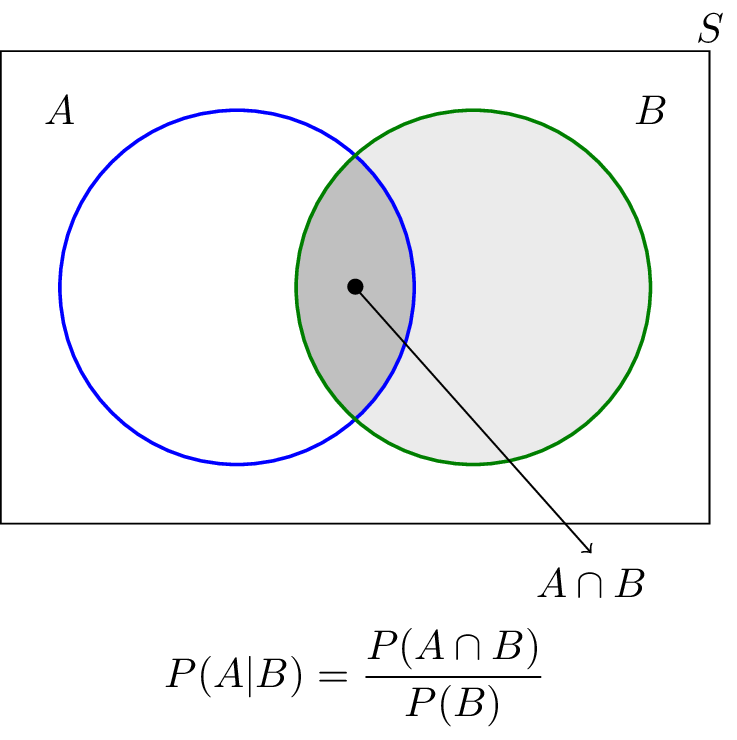
\includegraphics[width=0.7\linewidth]{conditional_b.png}
\end{center}

In formula if the non-default probability is indicated by \(N\) and the
hazard rate by \(\lambda\):

\[\lambda = -\frac{dN}{dt}\frac{1}{N(t_0, t_1)}\]

where the minus sign derives from the fact that \(N\) is a \textbf{non}
default probability while the hazard rate is defined in terms of the
probability of default.

Conversly given the hazard rate the non-default probability can be
determined as:

\[\lambda = -\frac{1}{dt}\cdot\frac{dN}{N} = -\frac{d(\textrm{log}N)}{dt}\]

\[N(t_0, t) = e^{-\int_{t_0}^{t}\lambda dt}\]

    \begin{Verbatim}[commandchars=\\\{\}]
{\color{incolor}In [{\color{incolor}3}]:} \PY{k+kn}{import} \PY{n+nn}{math}
        \PY{k+kn}{import} \PY{n+nn}{numpy}
        
        \PY{k}{class} \PY{n+nc}{CreditCurve}\PY{p}{(}\PY{n+nb}{object}\PY{p}{)}\PY{p}{:}
            
            \PY{k}{def} \PY{n+nf}{\PYZus{}\PYZus{}init\PYZus{}\PYZus{}}\PY{p}{(}\PY{n+nb+bp}{self}\PY{p}{,} \PY{n}{pillar\PYZus{}dates}\PY{p}{,} \PY{n}{pillar\PYZus{}ndps}\PY{p}{)}\PY{p}{:}
                
                \PY{n+nb+bp}{self}\PY{o}{.}\PY{n}{pillar\PYZus{}dates} \PY{o}{=} \PY{n}{pillar\PYZus{}dates}
                
                \PY{n+nb+bp}{self}\PY{o}{.}\PY{n}{pillar\PYZus{}days} \PY{o}{=} \PY{p}{[}
                    \PY{p}{(}\PY{n}{pd} \PY{o}{\PYZhy{}} \PY{n}{pillar\PYZus{}dates}\PY{p}{[}\PY{l+m+mi}{0}\PY{p}{]}\PY{p}{)}\PY{o}{.}\PY{n}{days}
                    \PY{k}{for} \PY{n}{pd} \PY{o+ow}{in} \PY{n}{pillar\PYZus{}dates}
                \PY{p}{]}
                
                \PY{n+nb+bp}{self}\PY{o}{.}\PY{n}{log\PYZus{}ndps} \PY{o}{=} \PY{p}{[}
                    \PY{n}{math}\PY{o}{.}\PY{n}{log}\PY{p}{(}\PY{n}{ndp}\PY{p}{)}
                    \PY{k}{for} \PY{n}{ndp} \PY{o+ow}{in} \PY{n}{pillar\PYZus{}ndps}
                \PY{p}{]}
                
            \PY{k}{def} \PY{n+nf}{ndp}\PY{p}{(}\PY{n+nb+bp}{self}\PY{p}{,} \PY{n}{value\PYZus{}date}\PY{p}{)}\PY{p}{:}
                
                \PY{n}{value\PYZus{}days} \PY{o}{=} \PY{p}{(}\PY{n}{value\PYZus{}date} \PY{o}{\PYZhy{}} \PY{n+nb+bp}{self}\PY{o}{.}\PY{n}{pillar\PYZus{}dates}\PY{p}{[}\PY{l+m+mi}{0}\PY{p}{]}\PY{p}{)}\PY{o}{.}\PY{n}{days}
                
                \PY{k}{return} \PY{n}{math}\PY{o}{.}\PY{n}{exp}\PY{p}{(}
                    \PY{n}{numpy}\PY{o}{.}\PY{n}{interp}\PY{p}{(}\PY{n}{value\PYZus{}days}\PY{p}{,}
                                 \PY{n+nb+bp}{self}\PY{o}{.}\PY{n}{pillar\PYZus{}days}\PY{p}{,}
                                 \PY{n+nb+bp}{self}\PY{o}{.}\PY{n}{log\PYZus{}ndps}\PY{p}{)}\PY{p}{)}
            
            \PY{k}{def} \PY{n+nf}{hazard}\PY{p}{(}\PY{n+nb+bp}{self}\PY{p}{,} \PY{n}{value\PYZus{}date}\PY{p}{)}\PY{p}{:}
                \PY{n}{ndp\PYZus{}1} \PY{o}{=} \PY{n+nb+bp}{self}\PY{o}{.}\PY{n}{ndp}\PY{p}{(}\PY{n}{value\PYZus{}date}\PY{p}{)}
                \PY{n}{ndp\PYZus{}2} \PY{o}{=} \PY{n+nb+bp}{self}\PY{o}{.}\PY{n}{ndp}\PY{p}{(}\PY{n}{value\PYZus{}date} \PY{o}{+} \PY{n}{relativedelta}\PY{p}{(}\PY{n}{days}\PY{o}{=}\PY{l+m+mi}{1}\PY{p}{)}\PY{p}{)}
                \PY{n}{delta\PYZus{}t} \PY{o}{=} \PY{l+m+mf}{1.0} \PY{o}{/} \PY{l+m+mf}{365.0}
                \PY{n}{h} \PY{o}{=} \PY{o}{\PYZhy{}}\PY{l+m+mf}{1.0} \PY{o}{/} \PY{n}{ndp\PYZus{}1} \PY{o}{*} \PY{p}{(}\PY{n}{ndp\PYZus{}2} \PY{o}{\PYZhy{}} \PY{n}{ndp\PYZus{}1}\PY{p}{)} \PY{o}{/} \PY{n}{delta\PYZus{}t}
                \PY{k}{return} \PY{n}{h}
\end{Verbatim}

    \begin{Verbatim}[commandchars=\\\{\}]
{\color{incolor}In [{\color{incolor}4}]:} \PY{k+kn}{from} \PY{n+nn}{datetime} \PY{k}{import} \PY{n}{date}
        \PY{k+kn}{from} \PY{n+nn}{dateutil}\PY{n+nn}{.}\PY{n+nn}{relativedelta} \PY{k}{import} \PY{n}{relativedelta}
        \PY{k+kn}{from} \PY{n+nn}{curve\PYZus{}data} \PY{k}{import} \PY{n}{pricing\PYZus{}date}
        
        \PY{n}{cc} \PY{o}{=} \PY{n}{CreditCurve}\PY{p}{(}
            \PY{p}{[}\PY{n}{pricing\PYZus{}date}\PY{p}{,} \PY{n}{pricing\PYZus{}date} \PY{o}{+} \PY{n}{relativedelta}\PY{p}{(}\PY{n}{years}\PY{o}{=}\PY{l+m+mi}{2}\PY{p}{)}\PY{p}{]}\PY{p}{,}
            \PY{p}{[}\PY{l+m+mf}{1.0}\PY{p}{,} \PY{l+m+mf}{0.8}\PY{p}{]}
        \PY{p}{)}
\end{Verbatim}

    \begin{Verbatim}[commandchars=\\\{\}]
{\color{incolor}In [{\color{incolor}5}]:} \PY{n}{cc}\PY{o}{.}\PY{n}{ndp}\PY{p}{(}\PY{n}{pricing\PYZus{}date} \PY{o}{+} \PY{n}{relativedelta}\PY{p}{(}\PY{n}{years}\PY{o}{=}\PY{l+m+mi}{1}\PY{p}{)}\PY{p}{)}
\end{Verbatim}

\begin{Verbatim}[commandchars=\\\{\}]
{\color{outcolor}Out[{\color{outcolor}5}]:} 0.8942906859183223
\end{Verbatim}
            
    \begin{Verbatim}[commandchars=\\\{\}]
{\color{incolor}In [{\color{incolor}6}]:} \PY{n}{cc}\PY{o}{.}\PY{n}{hazard}\PY{p}{(}\PY{n}{pricing\PYZus{}date} \PY{o}{+} \PY{n}{relativedelta}\PY{p}{(}\PY{n}{years}\PY{o}{=}\PY{l+m+mi}{1}\PY{p}{)}\PY{p}{)}
\end{Verbatim}

\begin{Verbatim}[commandchars=\\\{\}]
{\color{outcolor}Out[{\color{outcolor}6}]:} 0.11140214262993799
\end{Verbatim}
            
    \hypertarget{credit-deafult-swaps}{%
\subsection{Credit Deafult Swaps}\label{credit-deafult-swaps}}

Once we have implemented a \texttt{CreditCurve} class which allows us to
interpolate pillar non-default probabilities (NDPs) at arbitrary value
dates, and also allows us to calculate the hazard rate at an arbitrary
date, we can use it to price \textbf{credit default swaps} (CDSs).

CDSs are made up of two legs:

\begin{itemize}
\tightlist
\item
  the \emph{default} leg: which pays \(L = 1 - R\), known as the
  \textbf{loss given default} (LGD) if and when the credit event occurs,
  where \(R = 40\%\) is a conventional \textbf{recovery value};
\item
  the \emph{premium} leg: which pays \(S\) (\emph{spread}) every 3
  months until the credit event occurs.
\end{itemize}

\hypertarget{premium-leg}{%
\subsubsection{Premium leg}\label{premium-leg}}

Let's start with the premium leg, which is easier to calculate. We'll
use the following notation:

\begin{itemize}
\tightlist
\item
  \(d\) today's date
\item
  \(d_0\) the start date of the CDS (could be different from \(d\))
\item
  \(d_1, ..., d_n\) the payment dates of the premium leg, which occur at
  a 3-month frequency
\item
  we assume that \(d_n\) is the end date of the CDS
\item
  \(D(d')\) the discount factor between \(d\) and \(d'\)
\item
  \(N(d')\) the non-default probability between \(d\) and \(d'\)
\item
  \(\tau\) the random variable representing the date of the credit event
\end{itemize}

At each payment date \(d_i\), a flow of \(S\) is paid if and only if the
credit event has not occurred before that date. Therefore the NPV of the
each flow is

\[
\def\E{\mathbb{E}}
\def\1{\mathbb{1}}
\def\set#1{\!\left\{ #1 \right\}}
\tilde\E\left[ S \times D(d_i) \times \1\set{\tau > d_i} \right] = S \times D(d_i) \times N(d_i)
\]

therefore the NPV of the premium leg is simply the sum, over the payment
dates, of these terms:

\[\textrm{NPV}_{premium} = \sum_{i=1}^{n} S \times D(d_i) \times N(d_i)\]

\subsubsection{Default leg}\label{default-leg}

The LGD \(1-R\) is paid out on the same date on which the credit event
occurs, i.e.~it can potentially be paid out on any date between \(d_0\)
and \(d_n\). Mathematically, therefore, the NPV of the premium leg can
be expressed as follows:

\[
\tilde{\mathbb{E}}[(1-R) \times D(\tau) \times \mathbb{1} \{\tau \leq d_n\} ]
\]

Using the law of total probability, we can break this down into the sum
of ``daily NPVs'' calculated as a function of the daily forward default
probabilities:

\[
\begin{align*}
\tilde{\mathbb{E}}[(1-R) \times D(\tau) \times \mathbb{1}\{\tau \leq d_n\} ]
&= \sum_{d'=d_0}^{d_n} \tilde{\mathbb{E}}[ (1-R) \times D(\tau) \mid \tau = d'] \mathbb{P}[ \tau = d' ] \\
&= (1-R) \sum_{d'=d_0}^{d_n} D(d') \left( \mathbb{P}[ \tau \geq d' ] - \mathbb{P}[ \tau \geq d'+1 ] \right) \\
&= (1-R) \sum_{d'=d_0}^{d_n} D(d') \left( N(d') - N(d'+1) \right)
\end{align*}
\]

where the last step holds since $\mathbb{P}[\tau\geq d^{'}] = 1 - \mathbb{P}[\tau < d^{'}] = 1 - (1-N(d^{'})) = N(d^{'})$.

    \begin{Verbatim}[commandchars=\\\{\}]
{\color{incolor}In [{\color{incolor}7}]:} \PY{k+kn}{from} \PY{n+nn}{finmarkets} \PY{k}{import} \PY{n}{generate\PYZus{}swap\PYZus{}dates}
        
        \PY{k}{class} \PY{n+nc}{CreditDefaultSwap}\PY{p}{:}
            
            \PY{k}{def} \PY{n+nf}{\PYZus{}\PYZus{}init\PYZus{}\PYZus{}}\PY{p}{(}\PY{n+nb+bp}{self}\PY{p}{,} \PY{n}{notional}\PY{p}{,} \PY{n}{start\PYZus{}date}\PY{p}{,} \PY{n}{nyears}\PY{p}{,} \PY{n}{fixed\PYZus{}spread}\PY{p}{,} \PY{n}{recovery}\PY{o}{=}\PY{l+m+mf}{0.4}\PY{p}{)}\PY{p}{:}
                
                \PY{n+nb+bp}{self}\PY{o}{.}\PY{n}{notional} \PY{o}{=} \PY{n}{notional}
                \PY{n+nb+bp}{self}\PY{o}{.}\PY{n}{payment\PYZus{}dates} \PY{o}{=} \PY{n}{generate\PYZus{}swap\PYZus{}dates}\PY{p}{(}\PY{n}{start\PYZus{}date}\PY{p}{,} \PY{n}{nyears}\PY{o}{*}\PY{l+m+mi}{12}\PY{p}{,} \PY{l+m+mi}{3}\PY{p}{)}
                \PY{n+nb+bp}{self}\PY{o}{.}\PY{n}{fixed\PYZus{}spread} \PY{o}{=} \PY{n}{fixed\PYZus{}spread}
                \PY{n+nb+bp}{self}\PY{o}{.}\PY{n}{recovery} \PY{o}{=} \PY{n}{recovery}
            
            \PY{k}{def} \PY{n+nf}{premium\PYZus{}leg\PYZus{}npv}\PY{p}{(}\PY{n+nb+bp}{self}\PY{p}{,} \PY{n}{discount\PYZus{}curve}\PY{p}{,} \PY{n}{credit\PYZus{}curve}\PY{p}{)}\PY{p}{:}
                
                \PY{n}{npv} \PY{o}{=} \PY{l+m+mi}{0}
                
                \PY{k}{for} \PY{n}{i} \PY{o+ow}{in} \PY{n+nb}{range}\PY{p}{(}\PY{l+m+mi}{1}\PY{p}{,} \PY{n+nb}{len}\PY{p}{(}\PY{n+nb+bp}{self}\PY{o}{.}\PY{n}{payment\PYZus{}dates}\PY{p}{)}\PY{p}{)}\PY{p}{:}
                    \PY{n}{npv} \PY{o}{+}\PY{o}{=} \PY{p}{(}
                        \PY{n+nb+bp}{self}\PY{o}{.}\PY{n}{fixed\PYZus{}spread} \PY{o}{*}
                        \PY{n}{discount\PYZus{}curve}\PY{o}{.}\PY{n}{df}\PY{p}{(}\PY{n+nb+bp}{self}\PY{o}{.}\PY{n}{payment\PYZus{}dates}\PY{p}{[}\PY{n}{i}\PY{p}{]}\PY{p}{)} \PY{o}{*}
                        \PY{n}{credit\PYZus{}curve}\PY{o}{.}\PY{n}{ndp}\PY{p}{(}\PY{n+nb+bp}{self}\PY{o}{.}\PY{n}{payment\PYZus{}dates}\PY{p}{[}\PY{n}{i}\PY{p}{]}\PY{p}{)}
                    \PY{p}{)}
                    
                \PY{k}{return} \PY{n}{npv} \PY{o}{*} \PY{n+nb+bp}{self}\PY{o}{.}\PY{n}{notional}
            
            \PY{k}{def} \PY{n+nf}{default\PYZus{}leg\PYZus{}npv}\PY{p}{(}\PY{n+nb+bp}{self}\PY{p}{,} \PY{n}{discount\PYZus{}curve}\PY{p}{,} \PY{n}{credit\PYZus{}curve}\PY{p}{)}\PY{p}{:}
                
                \PY{n}{npv} \PY{o}{=} \PY{l+m+mi}{0}
                \PY{n}{d} \PY{o}{=} \PY{n+nb+bp}{self}\PY{o}{.}\PY{n}{payment\PYZus{}dates}\PY{p}{[}\PY{l+m+mi}{0}\PY{p}{]}
                
                \PY{k}{while} \PY{n}{d} \PY{o}{\PYZlt{}}\PY{o}{=} \PY{n+nb+bp}{self}\PY{o}{.}\PY{n}{payment\PYZus{}dates}\PY{p}{[}\PY{o}{\PYZhy{}}\PY{l+m+mi}{1}\PY{p}{]}\PY{p}{:}
                    
                    \PY{n}{npv} \PY{o}{+}\PY{o}{=} \PY{n}{discount\PYZus{}curve}\PY{o}{.}\PY{n}{df}\PY{p}{(}\PY{n}{d}\PY{p}{)} \PY{o}{*} \PY{p}{(}
                        \PY{n}{credit\PYZus{}curve}\PY{o}{.}\PY{n}{ndp}\PY{p}{(}\PY{n}{d}\PY{p}{)} \PY{o}{\PYZhy{}}
                        \PY{n}{credit\PYZus{}curve}\PY{o}{.}\PY{n}{ndp}\PY{p}{(}\PY{n}{d} \PY{o}{+} \PY{n}{relativedelta}\PY{p}{(}\PY{n}{days}\PY{o}{=}\PY{l+m+mi}{1}\PY{p}{)}\PY{p}{)}
                    \PY{p}{)}
                    
                    \PY{n}{d} \PY{o}{+}\PY{o}{=} \PY{n}{relativedelta}\PY{p}{(}\PY{n}{days}\PY{o}{=}\PY{l+m+mi}{1}\PY{p}{)}
                
                \PY{k}{return} \PY{n}{npv} \PY{o}{*} \PY{n+nb+bp}{self}\PY{o}{.}\PY{n}{notional} \PY{o}{*} \PY{p}{(}\PY{l+m+mi}{1} \PY{o}{\PYZhy{}} \PY{n+nb+bp}{self}\PY{o}{.}\PY{n}{recovery}\PY{p}{)}
            
            \PY{k}{def} \PY{n+nf}{npv}\PY{p}{(}\PY{n+nb+bp}{self}\PY{p}{,} \PY{n}{discount\PYZus{}curve}\PY{p}{,} \PY{n}{credit\PYZus{}curve}\PY{p}{)}\PY{p}{:}
                
                \PY{k}{return} \PY{n+nb+bp}{self}\PY{o}{.}\PY{n}{default\PYZus{}leg\PYZus{}npv}\PY{p}{(}\PY{n}{discount\PYZus{}curve}\PY{p}{,} \PY{n}{credit\PYZus{}curve}\PY{p}{)} \PY{o}{\PYZhy{}} \PYZbs{}
                       \PY{n+nb+bp}{self}\PY{o}{.}\PY{n}{premium\PYZus{}leg\PYZus{}npv}\PY{p}{(}\PY{n}{discount\PYZus{}curve}\PY{p}{,} \PY{n}{credit\PYZus{}curve}\PY{p}{)}
\end{Verbatim}

    \begin{Verbatim}[commandchars=\\\{\}]
{\color{incolor}In [{\color{incolor}8}]:} \PY{k+kn}{from} \PY{n+nn}{curve\PYZus{}data} \PY{k}{import} \PY{n}{discount\PYZus{}curve}\PY{p}{,} \PY{n}{pricing\PYZus{}date}
        \PY{k+kn}{from} \PY{n+nn}{dateutil}\PY{n+nn}{.}\PY{n+nn}{relativedelta} \PY{k}{import} \PY{n}{relativedelta}
        
        \PY{n}{credit\PYZus{}curve} \PY{o}{=} \PY{n}{CreditCurve}\PY{p}{(}\PY{p}{[}\PY{n}{pricing\PYZus{}date}\PY{p}{,} \PY{n}{pricing\PYZus{}date} \PY{o}{+} \PY{n}{relativedelta}\PY{p}{(}\PY{n}{months}\PY{o}{=}\PY{l+m+mi}{36}\PY{p}{)}\PY{p}{]}\PY{p}{,} 
                                   \PY{p}{[}\PY{l+m+mf}{1.0}\PY{p}{,} \PY{l+m+mf}{0.7}\PY{p}{]}\PY{p}{)}
        
        \PY{n}{cds} \PY{o}{=} \PY{n}{CreditDefaultSwap}\PY{p}{(}\PY{l+m+mf}{1e6}\PY{p}{,} \PY{n}{pricing\PYZus{}date}\PY{p}{,} \PY{l+m+mi}{3}\PY{p}{,} \PY{l+m+mf}{0.03}\PY{p}{)}
        \PY{n}{cds}\PY{o}{.}\PY{n}{premium\PYZus{}leg\PYZus{}npv}\PY{p}{(}\PY{n}{discount\PYZus{}curve}\PY{p}{,} \PY{n}{credit\PYZus{}curve}\PY{p}{)}
\end{Verbatim}

\begin{Verbatim}[commandchars=\\\{\}]
{\color{outcolor}Out[{\color{outcolor}8}]:} 300505.06774906756
\end{Verbatim}
            
    \begin{Verbatim}[commandchars=\\\{\}]
{\color{incolor}In [{\color{incolor}9}]:} \PY{n}{cds}\PY{o}{.}\PY{n}{default\PYZus{}leg\PYZus{}npv}\PY{p}{(}\PY{n}{discount\PYZus{}curve}\PY{p}{,} \PY{n}{credit\PYZus{}curve}\PY{p}{)}
\end{Verbatim}

\begin{Verbatim}[commandchars=\\\{\}]
{\color{outcolor}Out[{\color{outcolor}9}]:} 181369.30417135215
\end{Verbatim}
            
    \begin{Verbatim}[commandchars=\\\{\}]
{\color{incolor}In [{\color{incolor}10}]:} \PY{n}{cds}\PY{o}{.}\PY{n}{npv}\PY{p}{(}\PY{n}{discount\PYZus{}curve}\PY{p}{,} \PY{n}{credit\PYZus{}curve}\PY{p}{)}
\end{Verbatim}

\begin{Verbatim}[commandchars=\\\{\}]
{\color{outcolor}Out[{\color{outcolor}10}]:} -119135.7635777154
\end{Verbatim}
            
    \hypertarget{exercises}{%
\subsection{Exercises}\label{exercises}}

\hypertarget{exercise-7.1}{%
  \subsubsection{Exercise 7.1}\label{exercise-7.1}}

Update \verb!finmarkets! module with \verb!CreditCurve! and \verb!CreditDefaultSwap! classes.
    
\hypertarget{exercise-7.2}{%
\subsubsection{Exercise 7.2}\label{exercise-7.2}}

Applying a bootstrapping technique (outlined in lesson 5) derive the a
credit curve from the following CDS market quotes:

\begin{Shaded}
\begin{Highlighting}[]
\NormalTok{pricing_date }\OperatorTok{=}\NormalTok{ date(}\DecValTok{2019}\NormalTok{, }\DecValTok{11}\NormalTok{, }\DecValTok{6}\NormalTok{)}

\NormalTok{cds_quotes }\OperatorTok{=}\NormalTok{ [}
\NormalTok{    \{}\StringTok{'maturity'}\NormalTok{: }\DecValTok{12}\NormalTok{, }\StringTok{'spread'}\NormalTok{:}\FloatTok{0.0149}\NormalTok{\},}
\NormalTok{    \{}\StringTok{'maturity'}\NormalTok{: }\DecValTok{24}\NormalTok{, }\StringTok{'spread'}\NormalTok{:}\FloatTok{0.0165}\NormalTok{\},}
\NormalTok{    \{}\StringTok{'maturity'}\NormalTok{: }\DecValTok{36}\NormalTok{, }\StringTok{'spread'}\NormalTok{:}\FloatTok{0.0173}\NormalTok{\},}
\NormalTok{    \{}\StringTok{'maturity'}\NormalTok{: }\DecValTok{69}\NormalTok{, }\StringTok{'spread'}\NormalTok{:}\FloatTok{0.0182}\NormalTok{\},}
\NormalTok{    \{}\StringTok{'maturity'}\NormalTok{: }\DecValTok{120}\NormalTok{, }\StringTok{'spread'}\NormalTok{:}\FloatTok{0.0183}\NormalTok{\},}
\NormalTok{    \{}\StringTok{'maturity'}\NormalTok{: }\DecValTok{240}\NormalTok{, }\StringTok{'spread'}\NormalTok{:}\FloatTok{0.0184}\NormalTok{\},}
\NormalTok{]}
\end{Highlighting}
\end{Shaded}

\hypertarget{hint}{%
\paragraph{Hint}\label{hint}}

\begin{itemize}
\tightlist
\item
  create a CDS contract for each input market quote;
\item
  implement an objective function to minimize the squared sum of the CDS
  npvs, the function has to implement also a \texttt{CreditCurve} with
  the unknown (to be detrmined by the bootstrap survival probabilities)
  and a list of pillars corresponding to the CDS maturities;
\item
  remember to set initial guesses and boundary conditions for the
  unknown parameters (the first survival probability has to be set to 1
  since no default happened !, the others free to move between {[}0.01
  to 1{]});
\item
  using the \texttt{scipy.optimize.minimize} find the curve.
\end{itemize}

    \hypertarget{exercise-7.3}{%
\subsubsection{Exercise 7.3}\label{exercise-7.3}}

Using the above \texttt{Credit\ Curve} and the \texttt{DiscountCurve}
already defined in lesson 5, price the following CDS:

\begin{Shaded}
\begin{Highlighting}[]
\NormalTok{cds_to_price }\OperatorTok{=}\NormalTok{ [}
\NormalTok{    \{}\StringTok{'nominal'}\NormalTok{: }\DecValTok{5000000}\NormalTok{, }\StringTok{'maturity'}\NormalTok{: }\DecValTok{18}\NormalTok{, }\StringTok{'spread'}\NormalTok{: }\FloatTok{0.02}\NormalTok{\},}
\NormalTok{    \{}\StringTok{'nominal'}\NormalTok{: }\DecValTok{5000000}\NormalTok{, }\StringTok{'maturity'}\NormalTok{: }\DecValTok{30}\NormalTok{, }\StringTok{'spread'}\NormalTok{: }\FloatTok{0.02}\NormalTok{\},}
\NormalTok{    \{}\StringTok{'nominal'}\NormalTok{: }\DecValTok{5000000}\NormalTok{, }\StringTok{'maturity'}\NormalTok{: }\DecValTok{42}\NormalTok{, }\StringTok{'spread'}\NormalTok{: }\FloatTok{0.02}\NormalTok{\},}
\NormalTok{    \{}\StringTok{'nominal'}\NormalTok{: }\DecValTok{5000000}\NormalTok{, }\StringTok{'maturity'}\NormalTok{: }\DecValTok{72}\NormalTok{, }\StringTok{'spread'}\NormalTok{: }\FloatTok{0.02}\NormalTok{\},}
\NormalTok{    \{}\StringTok{'nominal'}\NormalTok{: }\DecValTok{5000000}\NormalTok{, }\StringTok{'maturity'}\NormalTok{: }\DecValTok{108}\NormalTok{, }\StringTok{'spread'}\NormalTok{: }\FloatTok{0.02}\NormalTok{\},}
\NormalTok{    \{}\StringTok{'nominal'}\NormalTok{: }\DecValTok{5000000}\NormalTok{, }\StringTok{'maturity'}\NormalTok{: }\DecValTok{132}\NormalTok{, }\StringTok{'spread'}\NormalTok{: }\FloatTok{0.02}\NormalTok{\},}
\NormalTok{    \{}\StringTok{'nominal'}\NormalTok{: }\DecValTok{5000000}\NormalTok{, }\StringTok{'maturity'}\NormalTok{: }\DecValTok{160}\NormalTok{, }\StringTok{'spread'}\NormalTok{: }\FloatTok{0.02}\NormalTok{\},}
\NormalTok{    \{}\StringTok{'nominal'}\NormalTok{: }\DecValTok{5000000}\NormalTok{, }\StringTok{'maturity'}\NormalTok{: }\DecValTok{184}\NormalTok{, }\StringTok{'spread'}\NormalTok{: }\FloatTok{0.02}\NormalTok{\},}
\NormalTok{    \{}\StringTok{'nominal'}\NormalTok{: }\DecValTok{5000000}\NormalTok{, }\StringTok{'maturity'}\NormalTok{: }\DecValTok{210}\NormalTok{, }\StringTok{'spread'}\NormalTok{: }\FloatTok{0.02}\NormalTok{\}}
\NormalTok{]}
\end{Highlighting}
\end{Shaded}


    % Add a bibliography block to the postdoc
    
    
    
    \end{document}
